\documentclass[a4paper,14pt]{extarticle}

\usepackage[utf8x]{inputenc}
\usepackage[T1,T2A]{fontenc}
\usepackage[russian]{babel}
\usepackage{hyperref}
\usepackage{indentfirst}
\usepackage{here}
\usepackage{array}
\usepackage{graphicx}
\usepackage{caption}
\usepackage{subcaption}
\usepackage{chngcntr}
\usepackage{amsmath}
\usepackage{amssymb}
\usepackage{pgfplots}
\usepackage{pgfplotstable}
\usepackage[left=2cm,right=2cm,top=2cm,bottom=2cm,bindingoffset=0cm]{geometry}
\usepackage{multicol}
\usepackage{askmaps}
\usepackage{enumitem}

\setitemize{itemsep=0em}
\setenumerate{itemsep=0em}

\renewcommand{\le}{\ensuremath{\leqslant}}
\renewcommand{\leq}{\ensuremath{\leqslant}}
\renewcommand{\ge}{\ensuremath{\geqslant}}
\renewcommand{\geq}{\ensuremath{\geqslant}}
\renewcommand{\epsilon}{\ensuremath{\varepsilon}}
\renewcommand{\phi}{\ensuremath{\varphi}}
\renewcommand{\thefigure}{\arabic{figure}} 	
\renewcommand*\not[1]{\overline{#1}}

%\titleformat*{\section}{\large\bfseries} 
%\titleformat*{\subsection}{\normalsize\bfseries} 
%\titleformat*{\subsubsection}{\normalsize\bfseries} 
%\titleformat*{\paragraph}{\normalsize\bfseries} 
%\titleformat*{\subparagraph}{\normalsize\bfseries} 

\counterwithin{figure}{section}
\counterwithin{equation}{section}
\counterwithin{table}{section}
\newcommand{\sign}[1][5cm]{\makebox[#1]{\hrulefill}}
\graphicspath{{../pics/}}
\captionsetup{justification=centering,margin=1cm}
\def\arraystretch{1.3}
\setlength\parindent{5ex}
%\titlelabel{\thetitle.\quad}

\begin{document}

\begin{titlepage}
\begin{center}
	Санкт-Петербургский Политехнический Университет Петра Великого\\[0.3cm]
	Институт компьютерных наук и технологий \\[0.3cm]
	Кафедра компьютерных систем и программных технологий\\[4cm]
	
	\textbf{ОТЧЕТ}\\ 
	\textbf{по лабораторной работе}\\[0.5cm]
	\textbf{<<Исследование персептронов>>}\\[0.1cm]
	\textbf{Нейроинформатика}\\[4.0cm]
\end{center}

\begin{flushright}
	\begin{minipage}{0.45\textwidth}
		\textbf{Работу выполнил студент}\\[3mm]
		группа 33501/4 \hspace*{10mm} Дьячков В.В.\\[5mm]
		\textbf{Преподаватель}\\[5mm]
		\sign[1.7cm] \hspace*{1mm} к.т.н., доц. Никитин К.В. \\[5mm]
	\end{minipage}
\end{flushright}

\vfill

\begin{center}
	Санкт-Петербург\\
	\the\year
\end{center}
\end{titlepage}

\addtocounter{page}{1}

\tableofcontents
\newpage
\listoffigures
\newpage

\section{Цели работы}

Изучение архитектуры статических и динамических линейных нейронных сетей и специальных функций для их создания, обучения по правилу Уидроу–Хоффа, приобретение навыков построения и обучения линейных сетей для классификации векторов, линейной аппроксимации, предсказания и фильтрации сигналов, идентификации и моделирования линейных систем.

\section{Аппроксимация нелинейной зависимости}

\subsection{Обучающая выборка}

%1. Сформируйте обучающую и тестовую выборки для задачи аппроксимации 1-мерной нелинейной зависимости (варианты с номером 5). 

На рис. \ref{fig:1_1} изображена сформированная обучающая выборка для задача аппроксимации.

\begin{figure}[H]
\begin{center}
	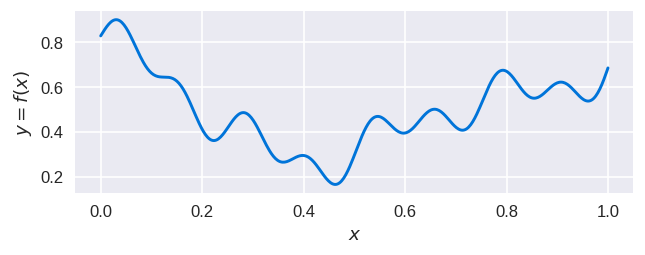
\includegraphics[scale=1]{1_1}
	\caption{Обучающая выборка}
	\label{fig:1_1}
\end{center}
\end{figure}

\subsection{Обучение линейной нейронной сети}

%2. Создайте линейную НС и обучите ее на обучающей выборке. Постройте графики зависимостей, реализуемых НС на различных этапах обучения на одном графике с исходной зависимостью. Оцените ошибку аппроксимации (абсолютную и относительную) на обучающей и тестовой выборках.
%3. Создайте НС и одновременно обучите ее в соответствии с МНК с помощью функции newlind. Сравните результаты (результирующую функцию и ошибки) с предыдущим вариантом.

На рис. \ref{fig:1_2_1} изображены зависимости, реализуемые НС на различных этапах обучения.
\begin{figure}[H]
\begin{center}
	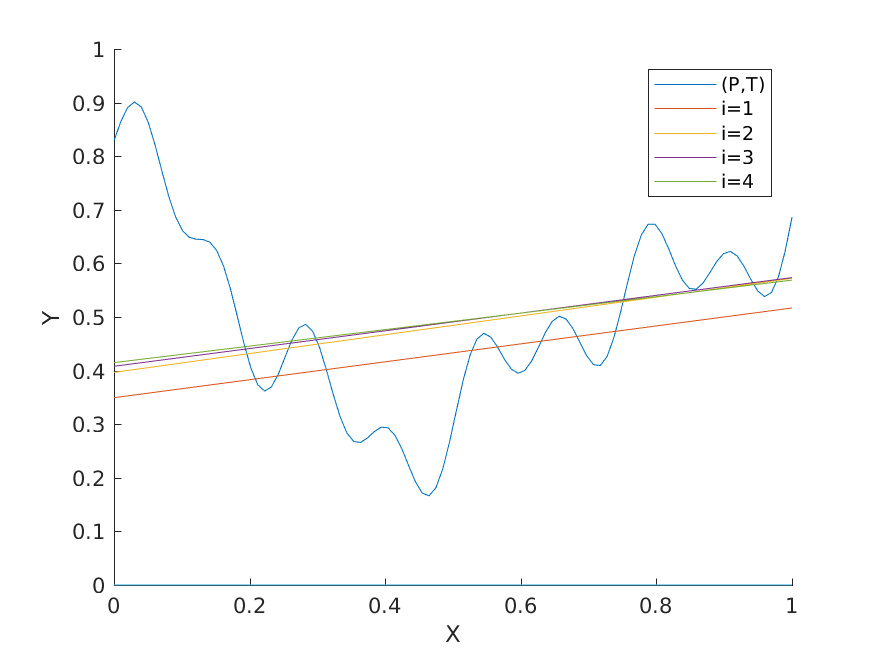
\includegraphics[scale=1]{1_2_1}
	\caption{Зависимости, реализуемые НС на различных этапах обучения}
	\label{fig:1_2_1}
\end{center}
\end{figure}

На рис. \ref{fig:1_2_2} изображена аппроксимация, полученная после обучения нейронной сети, в соответствии с МНК с помощью функции \verb+newlind+.
\begin{figure}[H]
\begin{center}
	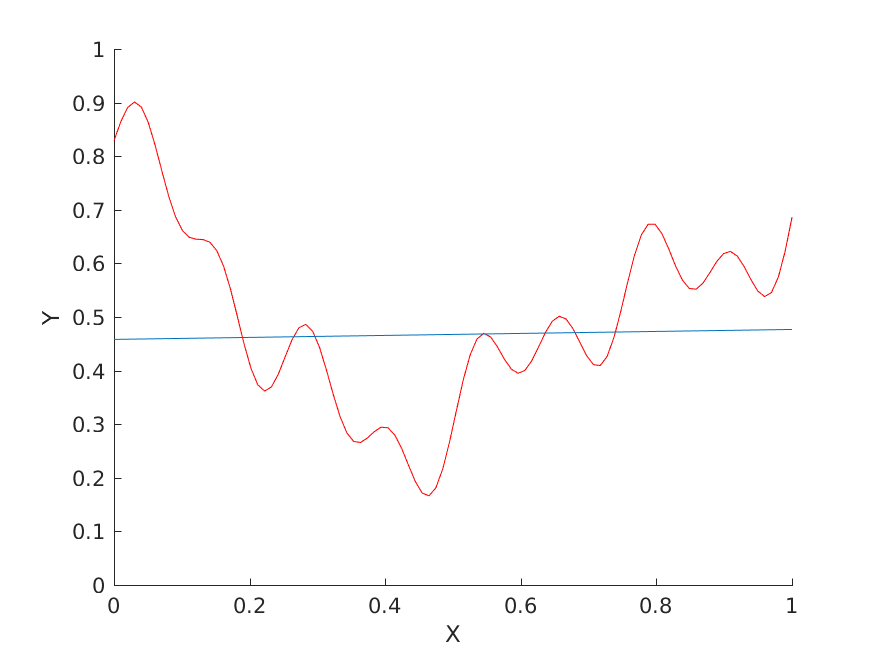
\includegraphics[scale=1]{1_2_2}
	\caption{Зависимости, реализуемые НС на различных этапах обучения}
	\label{fig:1_2_2}
\end{center}
\end{figure}

Из полученных результатов видно, что линейная нейронная сеть не может аппроксимировать нелинейную функцию.

\section{Классификация}

%Обучите линейную НС классификации сложных образов (варианты с номером 3) по аналогии с примером 4. Подберите значение порога threshold, обеспечивающее минимальную среднюю ошибку. Постройте результирующее разбиение плоскости на классы и приведите среднюю ошибку.

\subsection{Набор входных и желаемых образов}

Сформируем набор входных и желаемых выходных образов для двух линейно-неразделимых классов. На рис. \ref{fig:2_1} входной набор изоражен на графике, при этом класс \verb+1+ выделен синей областью.

\begin{figure}[H]
\begin{center}
	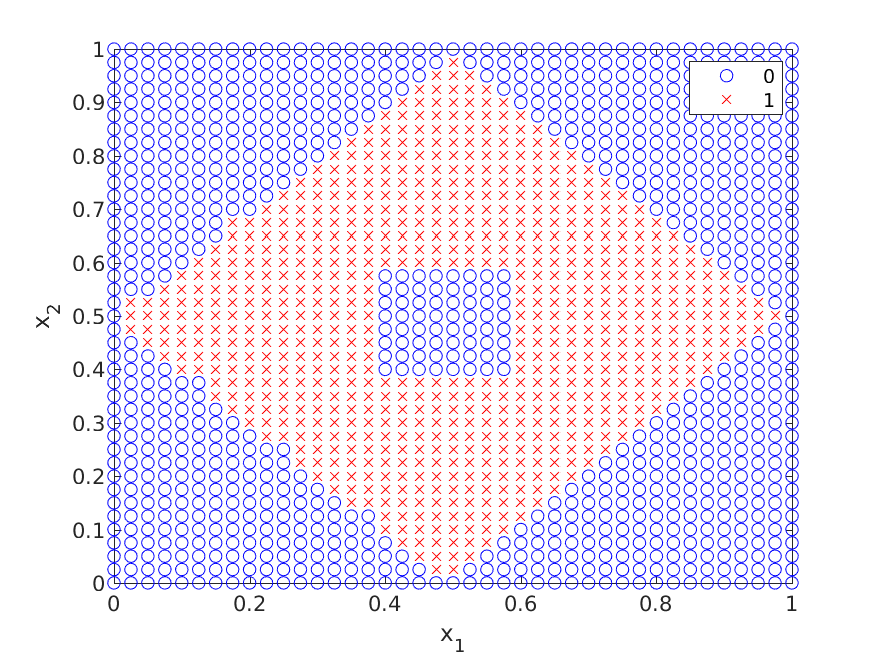
\includegraphics[scale=1]{2_1}
	\caption{Набор входных и желаемых выходных образов}
	\label{fig:2_1}
\end{center}
\end{figure}

\subsection{Обучение линейное нейронной сети}

На рис. \ref{fig:2_2} изображено разбиение точек входного пространства на классы при помощи обученной линейной нейронной сети. При этом средняя ошибка на обучаяющей выборке $E_{train} = 0.5463$, а на тестовой $E_{test} = 0.5833$.
\begin{figure}[H]
\begin{center}
	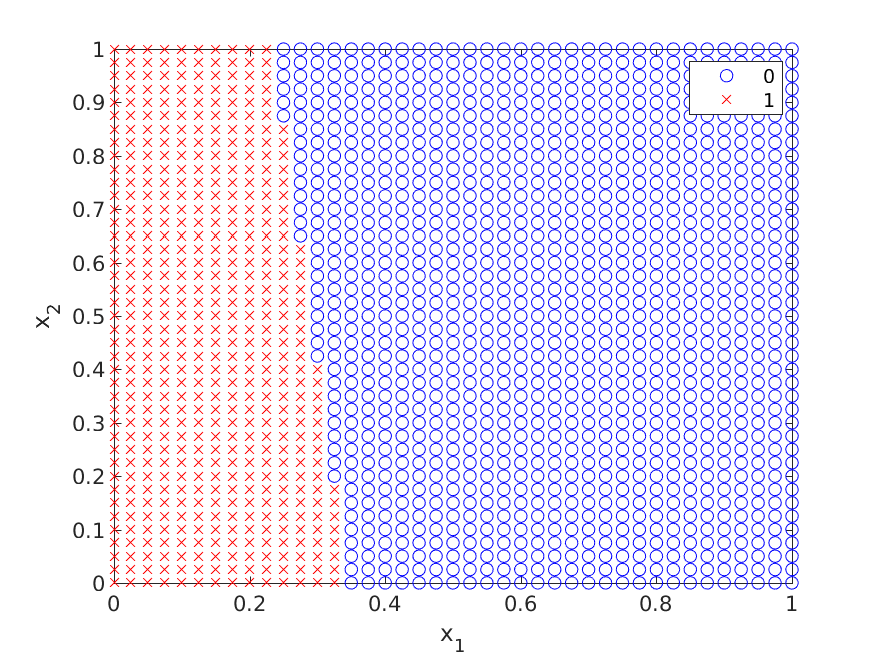
\includegraphics[scale=1]{2_2}
	\caption{Разбиение на классы}
	\label{fig:2_2}
\end{center}
\end{figure}

Из полученных результатов видно, что линейная нейронная сеть не может классифицировать линейно неразделимые классы.

\section{Выбор скорости обучения}

%Сформируйте обучающую выборку для функции (варианты с номером 5). Определите максимальную скорость обучения с помощью функции maxlinlr (разберитесь с принципом определения этой скорости). Проверьте, является ли эта скорость максимальной и если нет, то экспериментальным путем определите максимально допустимую скорость обучения. Затем проведите последовательность экспериментов для трех вариантов (скорость обучения а) больше (1 значение), б) равна (1 значение), в) меньше максимально допустимой (3 значения):
%1. Задайте фиксированные начальные значениями [W,b].
%2. Проведите обучение на достаточном числе циклов обучения. Постройте график изменения вектора [W,b] в течение обучения на графике поверхности (линий равного уровня) ошибок.
%Сравните результаты. Определите значение скорости обучения, при которой обучение проходит быстрее всего.

На рис. \ref{fig:2_3} изображены значения вектора \verb+[W, b]+ на графике поверхности ошибок и реализуемой функции в зависимости от скорости обучения $\alpha$.

\begin{figure}[H]
\begin{center}
	\begin{subfigure}[b]{0.49\textwidth}
		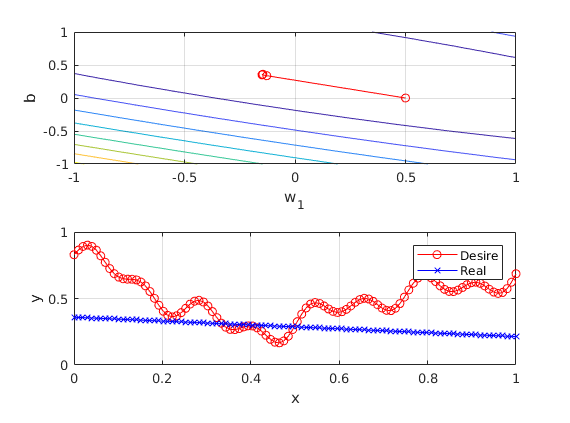
\includegraphics[width=1.1\textwidth]{2_3_1}
		\caption{$\alpha = 5$}
	\end{subfigure}
	\begin{subfigure}[b]{0.49\textwidth}
		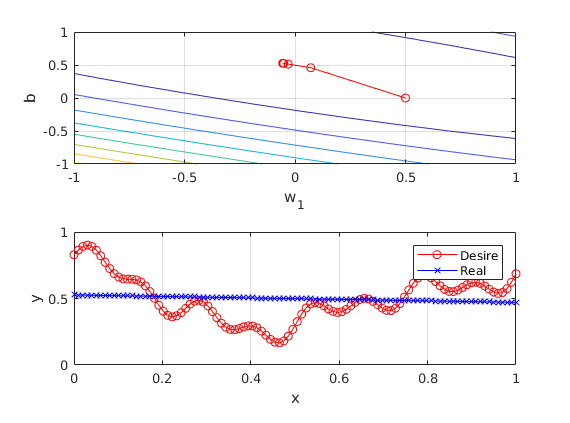
\includegraphics[width=1.1\textwidth]{2_3_2}
		\caption{$\alpha = 1$}
	\end{subfigure}
	\begin{subfigure}[b]{0.49\textwidth}
		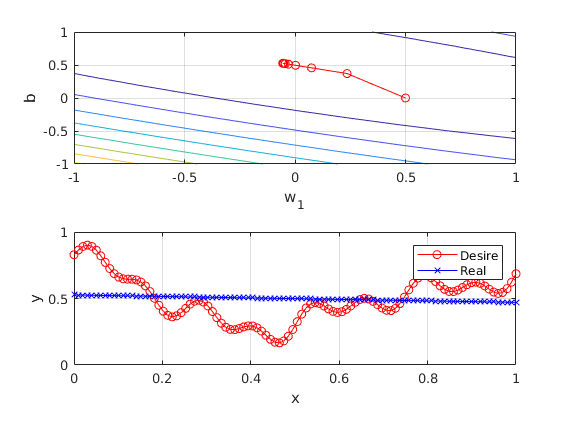
\includegraphics[width=1.1\textwidth]{2_3_3}
		\caption{$\alpha = 0.5$}
	\end{subfigure}
	\begin{subfigure}[b]{0.49\textwidth}
		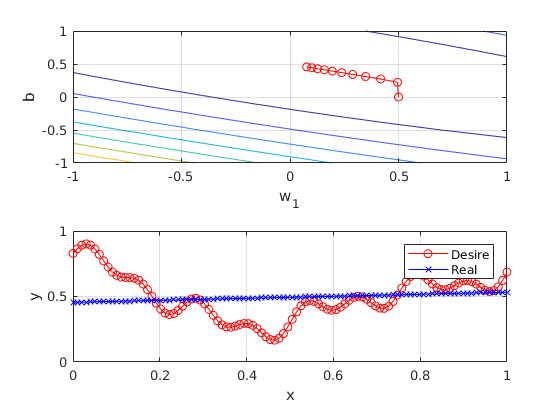
\includegraphics[width=1.1\textwidth]{2_3_4}
		\caption{$\alpha = 0.1$}
	\end{subfigure}
	\begin{subfigure}[b]{0.49\textwidth}
		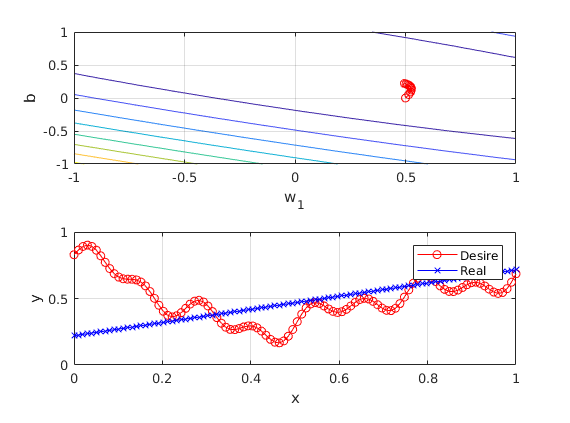
\includegraphics[width=1.1\textwidth]{2_3_5}
		\caption{$\alpha = 0.01$}
	\end{subfigure}
	\caption{Значения вектора W, b и реализуемой функции в зависимости от скорости обучения}
	\label{fig:2_3}
\end{center}
\end{figure}

Из графиков видно, что обучение проходит быстрее всего при $\alpha = 1$, т.е. при скорости обучения, определенной с помощью функции \verb+maxlinlr+. При этом если скорость обучения будет сильно меньше или сильно больше этого значения, то сеть будет обучаться слишком медленно, или не будет обучаться вовсе. Небольшое увелечение или уменьшение этого параметра приведет к увелечению числа шагов обучения.

\section{Многослойная линейная сеть}

%Покажите математически, что многослойная линейная сеть эквивалентна однослойной линейной НС. 

Однослойная линейная сеть обладает такими же способностями к обучению, как и многослойная. Для любой многослойной линейной сети существует эквивалентная однослойная линейная нейронная сеть, так как передаточная функция каждого нейроная является линейной, т.е. $\alpha = \verb+purelin+(n) = \verb+purelin+(Wp+b) = Wp+b$. Рассмотрим двухслойную и однослойную линейные сети.

\begin{figure}[H]
\begin{center}
	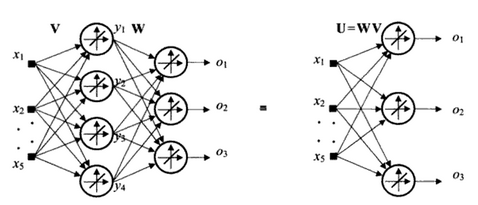
\includegraphics[scale=0.8]{2_4}
	\caption{Однослойная и двухслойная линейные сети}
	\label{fig:2_4}
\end{center}
\end{figure}

Из-за линейной передаточной функии двухслойная линейная сеть описывается двумя матрицами трансформации:
\begin{equation*}
y = Vx,\ o = Wy,
\end{equation*}
где $V$ -- матрица весов скрытого слоя, а $W$ -- матрица весов выходного слоя. Если подставить во второе уравнение значение $y$ из первого, то получим:
\begin{equation*}
o = W(Vx) = Ux,
\end{equation*}
где $U$ -- произведение матриц $W$ и $V$. Таким образом, однослойная нейронная сеть эквивалентна двухслойной.

Таким образом, чтобы перейти от многослойной к эквивалентной однослойной нейронной сети, достаточно установить матрицу весов однослойной сети, равной произведению матриц весов многослойной линейнной сети. 

\section{Выводы}

В данной работе были приобретены навыки построения и обучения линейных сетей для классификации сложных образов и линейной аппроксимации. Была изучена архитектура статических и динамических линейных нейронных сетей и специальных функций для их создания.

\end{document}